\documentclass[10pt]{article}
\usepackage[margin=1in, paperwidth=8.5in, paperheight=11in]{geometry}
\usepackage{ifpdf, amsmath, amssymb, comment, color, graphicx, stmaryrd, setspace, enumitem, fancyhdr, wrapfig, textcomp, mathptmx, siunitx, multicol}
\usepackage{hyperref}
\hypersetup{
    colorlinks=true,
    urlcolor=blue,
}

\usepackage{tikz}
\usetikzlibrary{trees}

\setlength{\headheight}{14.5pt}
\newcommand{\del}{\nabla}
\newcommand{\Q}{\mathbb{Q}}
\newcommand{\R}{\mathbb{R}}
\newcommand{\Z}{\mathbb{Z}}
\newcommand{\vu}{\mathbf{u}}
\newcommand{\vv}{\mathbf{v}}
\newcommand{\vw}{\mathbf{w}}
\newcommand{\vi}{\mathbf{i}}
\newcommand{\vj}{\mathbf{j}}
\newcommand{\vk}{\mathbf{k}}
\newcommand{\vn}{\mathbf{n}}
\newcommand{\vr}{\mathbf{r}}
\newcommand{\vs}{\mathbf{s}}
\newcommand{\va}{\mathbf{a}}
\newcommand{\vF}{\mathbf{F}}
\newcommand{\vL}{\mathbf{L}}
\newcommand{\vT}{\mathbf{T}}
\newcommand{\vN}{\mathbf{N}}
\newcommand{\vB}{\mathbf{B}}
\newcommand{\comp}{\operatorname{comp}}
\newcommand{\proj}{\operatorname{proj}}
\newcommand{\orth}{\operatorname{orth}}
\newcommand\dotp[1][.5]{\,\mathbin{\vcenter{\hbox{\scalebox{#1}{$\bullet$}}}}\,}


\newenvironment{red}{\color{red}}{\ignorespacesafterend}
\newcommand{\blue}[1]{\textcolor{blue}{#1}}
\newcommand{\green}[1]{\textcolor{green}{#1}}
\renewcommand{\section}[1]{\begin{center} \textbf{#1} \\\end{center}}
%
\hyphenpenalty=5000
\setlength{\parindent}{0in}
%\oddsidemargin=-.25in
\allowdisplaybreaks
\pagestyle{fancy}
\renewcommand{\headrulewidth}{0pt}
\lhead{MATH 203}
\rhead{Fall 2024}
%\lfoot{}
%\cfoot{}

\begin{document}
%


%\onehalfspacing
\allowdisplaybreaks
%##################################################################
\section{PS\#4: Calculus with space curves - \red{Answer key} }

\begin{enumerate}[leftmargin=0pt]

\item (\href{https://activecalculus.org/multi/S-9-7-Vector-Valued-Functions-Derivatives.html#Ez_9_7_1}{AC Multi 9.7 Exercise 13}) Compute the derivative of each of the following functions in two different ways: (1) use the rules provided in the theorem stated just after Activity 9.7.3, and (2) rewrite each given function so that it is stated as a single function (either a scalar function or a vector-valued function with three components), and differentiate component-wise. Compare your answers to ensure that they are the same.
\begin{enumerate}
    \item $\displaystyle \vr(t) = \sin(t) \langle 2t, t^2, \arctan(t) \rangle$
    
    \begin{red}
        Using the scalar product rule:
        \begin{align*}
            \frac{d\vr}{dt} &= \left(\dfrac{d}{dt}\sin(t)\right) 
            \langle 2t, t^2, \arctan(t) \rangle
            + \sin(t)
            \left(\dfrac{d}{dt} \langle 2t, t^2, \arctan(t) \rangle\right) \\
            &= \cos(t) \langle 2t, t^2, \arctan(t) \rangle
            + \sin(t) \left\langle 2, 2t, \dfrac{1}{1+t^2} \right\rangle \\
            &= \left\langle 2t\cos(t) + 2\sin(t),
                            t^2\cos(t)+2t\sin(t),
                            \arctan(t) \cos(t) + \dfrac{\sin(t)}{1+t^2} \right\rangle
        \end{align*}
        And rewriting first:
        \begin{align*}
            \vr(t) &= \langle 2t \sin(t) , t^2 \sin(t) , \arctan(t) \sin(t)  \rangle \\
            \frac{d\vr}{dt} &= \left\langle
                    \left(\frac{d}{dt} 2t\right) \sin(t) + 2t \left(\frac{d}{dt}\sin(t)\right),
                    \left(\frac{d}{dt}t^2\right)\sin(t) + t^2 \left(\frac{d}{dt}\sin(t)\right),
                    \left(\frac{d}{dt}\arctan(t)\right) \sin(t) + \arctan(t) \left(\frac{d}{dt} \sin(t) \right)
                \right\rangle \\
                &= \left\langle 2t\cos(t) + 2\sin(t),
                t^2\cos(t)+2t\sin(t),
                \dfrac{\sin(t)}{1+t^2} + \arctan(t) \cos(t) \right\rangle
        \end{align*}
    \end{red}

    \item $\vs(t) = \vr(2^t)$, where $\vr(t) = \langle t+2, \ln(t), 1 \rangle$ \begin{red}
        -- Note that $\vr'(t) = \langle 1, \frac1t, 0 \rangle$
    \end{red}
    
    \begin{red}
        Using the chain rule first:
        \begin{align*}
            \vs'(t) &= \vr'(2^t)\, \frac{d}{dt}2^t \\
            &=\left\langle 1, \dfrac{1}{2^t}, 0\right\rangle
            \, 2^t \ln(2) \\
            &= \left\langle 2^t \ln(2), \ln(2), 0 \right\rangle
        \end{align*}
        And simplifying first:
        \begin{align*}
            \vs(t) &= \vr(2^t) = \langle 2^t + 2, \ln(2^t), 1\rangle 
            = \langle 2^t + 2, t\ln(2), 1\rangle \\
            \vs'(t) &= \langle 2^t \ln(2), \ln(2), 0 \rangle
        \end{align*}
    \end{red}
    \item $\displaystyle \vr(t) = \langle \cos(t), \sin(t), t \rangle \dotp \langle -\sin(t), \cos(t), 1 \rangle$
    
    \begin{red}
        Using the dot product rule:
        \begin{align*}
            r'(t) &= \left(\frac{d}{dt}\langle \cos(t), \sin(t), t \rangle \right)\dotp \langle -\sin(t), \cos(t), 1 \rangle
            + \langle \cos(t), \sin(t), t \rangle \dotp \left(\frac{d}{dt} \langle -\sin(t), \cos(t), 1 \rangle\right) \\
            &= \langle -\sin(t), \cos(t), 1 \rangle \dotp \langle -\sin(t), \cos(t), 1 \rangle 
            + \langle \cos(t), \sin(t), t \rangle \dotp \langle -\cos(t), -\sin(t), 0\rangle \\
            &= \left[ \sin^2(t) + \cos^2(t) + 1 \right]
            + \left[ -\cos^2(t) -\sin^2(t) + 0\right] = 1 + 1 - 1 + 0 = 1 (!!)
        \end{align*}
        And rewriting first:
        \begin{align*}
            r(t) &= cos(t)\cdot(-\sin(t)) + \sin(t)\cdot\cos(t) + t\cdot 1 \\
            r(t) &= t \, (!!) \\
            r'(t) &= 1
        \end{align*}
    \end{red}
    \item $\displaystyle \vr(t) = \langle \cos(t), \sin(t), t \rangle \times \langle -\sin(t), \cos(t), 1 \rangle$
    
    \begin{red}
        Using the cross product rule:
        \begin{align*}
            \vr'(t) &= \left(\dfrac{d}{dt} \langle \cos(t), \sin(t), t \rangle \right)\times 
            \langle -\sin(t), \cos(t), 1 \rangle
            + \langle \cos(t), \sin(t), t \rangle \times 
            \left(\dfrac{d}{dt} \langle -\sin(t), \cos(t), 1 \rangle \right) \\
            &= \langle -\sin(t), \cos(t), 1 \rangle
            \times \langle -\sin(t), \cos(t), 1 \rangle
            + \langle \cos(t), \sin(t), t \rangle
            \times \langle -\cos(t), -\sin(t), 0 \rangle \\
            \intertext{The first two vectors are parallel, so their cross product is $\mathbf{0}$.}
            &= \mathbf{0} + \langle \cos(t), \sin(t), t \rangle
            \times \langle -\cos(t), -\sin(t), 0 \rangle 
            = \langle t\sin(t), -t\cos(t), 0 \rangle \quad\text{ (Thanks, WA!)}
        \end{align*}
        And finding the cross product first:
        \begin{align*}
            \vr(t) &= \langle \sin(t) - t\cos(t), -t\sin(t) - \cos(t), \sin^2(t) + \cos^2(t)\rangle 
            = \langle \sin(t) - t\cos(t), -t\sin(t) - \cos(t), 1 \rangle \\
            \vr'(t) &= \dfrac{d}{dt} \langle \sin(t) - t\cos(t), -t\sin(t) - \cos(t), 1 \rangle \\
            &= \langle \cos(t) - (1 \cos(t) + t(-\sin(t))),
            -(1\sin(t) + t\cos(t)) - (-\sin(t)), 0 \rangle \\
            &= \langle t\sin(t), -t\cos(t), 0 \rangle
        \end{align*}
    \end{red}
\end{enumerate}

\item (\href{https://activecalculus.org/multi/S-9-7-Vector-Valued-Functions-Derivatives.html#Ez_9_7_6}{AC Multi 9.7 Exercise 18}) A central force is one that acts on an object so that the force $\vF$ is parallel to the object's position $\vr$. Since Newton's Second Law says that an object's acceleration is proportional to the force exerted on it, the acceleration $\va$ of an object moving under a central force will be parallel to its position $\vr$. For instance, the Earth's acceleration due to the gravitational force that the sun exerts on the Earth is parallel to the Earth's position vector (see figure in the textbook).
	    
\begin{enumerate}
    \item If an object of mass $m$ is moving under a central force, the angular momentum vector is defined to be $\vL = m\vr \times \vv$. Assuming the mass is constant, show that the angular momentum is constant by showing that $\frac{d\vL}{dt} = \mathbf{0}$.
    
    \begin{red}
    Some stuff to keep track of: 
    \begin{itemize}
        \item $m$ is a constant scalar;
        \item $\vr$ is a variable vector (depends on $t$);
        \item $\vv$ is a variable vector (depends on $t$).
    \end{itemize} 
    Seems like the natural thing to do is to use the product rule to compute $\frac{d\vL}{dt}$:
    \begin{align*}
        \frac{d\vL}{dt} &= \frac{d}{dt}\left[m\vr\times\vv \right]
        = \frac{d}{dt}\left[ m\vr \right] \times \vv + 
        m\vr \times \frac{d}{dt} \left[ \vv \right] \\
        \intertext{Well, the derivative of position is velocity, and the derivative of velocity is acceleration:}
        &= [m\vv] \times \vv + m\vr \times \va \\
        \intertext{Now we're getting somewhere. Remember that the cross product of two parallel vectors is $\mathbf 0$. $m\vv$ is certainly parallel to $\vv$, and we're assuming in the context of the problem that $\va$ is parallel to $\vr$, so it's also parallel to $m\vr$. }
        &= \mathbf 0 + \mathbf 0 = \mathbf 0.
    \end{align*}
    Cool, so that tells us that $\vL$ is a constant vector.
    \end{red}
    
    \item Explain why $\vL \dotp \vr = 0$.
    
    \begin{red} 
    $\vL$ was defined as the cross product of $m\vr$ and $\vv$, so it's perpendicular to both of those. Since $m$ is a scalar, $m\vr$ points in the same direction as $\vr$, so if $\vL$ is perpendicular to $m\vr$, it's also perpendicular to $\vr$. Therefore, their dot product is zero.
    \end{red}
    
    \item Explain why we may conclude that the object is constrained to lie in the plane passing through the origin and perpendicular to $\vL$.
    
    \begin{red}
    The equation $\vL \dotp \vr = 0$ reminds me of the vector equation of a plane, with $\vL$ as the (constant) normal vector and $\vr$ playing the role of $\overrightarrow{PP_0}$. Since $\vr$'s initial point is the origin, we thus have the plane that's perpendicular to $\vL$ and passing through the origin.
    
    (Another way to see this: Certainly all the position vectors are perpendicular to $\vL$. Also, certainly all the position vectors emanate from the origin. Also, we've just found that $\vL$ is constant. So the only way this is going to happen is if all the position vectors lie in the \textbf{same} plane -- specifically, the plane containing the origin and perpendicular to the constant vector $\vL$.)
    \end{red}
\end{enumerate}

\item (\href{https://activecalculus.org/multi/S-9-8-Arc-Length-Curvature.html#Ez_9_8_4}{AC Multi 9.8 Exercise 14}) Consider the standard helix parameterized by $\vr(t) = \cos(t) \vi + \sin(t) \vj + t \vk$.
\begin{enumerate}
    \item Recall that the unit tangent vector $\vT(t)$ is the vector tangent to the curve at time $t$ that points in the direction of motion and has length 1. Find $\vT(t)$.
    \begin{red}
        \begin{align*}
            \vr'(t) &= \langle -\sin(t), \cos(t), 1 \rangle \\
            |\vr'(t)| &= \left[\sin^2(t) + \cos^2(t) + 1^2\right] = \sqrt{2} \\
            \vT(t) = \dfrac{\vr'(t)}{|\vr'(t)|} &= \dfrac{1}{\sqrt{2}} \langle -\sin(t), \cos(t), 1 \rangle
        \end{align*}
    \end{red}
    \item Explain why the fact that $|\vT(t)|=1$ implies that $\vT$ and $\vT'$ are orthogonal vectors for every value of $t$. 

    \begin{red}
        The hint is to look at the dot product of $\vT$ and $\vT'$. Where would that have come from? Well, certainly if we did the derivative of $\vT \dotp \vT$, then the product rule would make that pop out:
        $\dfrac{d}{dt} [\vT\dotp\vT] = \vT' \dotp \vT + \vT \dotp \vT'$. But since $\vT' \dotp \vT = \vT \dotp \vT'$, this is $2(\vT\dotp \vT')$.

        The other thing we know about a dot product of a vector with itself is that it's the magnitude of that vector squared: $\vT \dotp \vT = |\vT|^2 = 1^2 = 1$. Therefore, its derivative must be zero.

        So now let's combine the two things we know about $\dfrac{d}{dt}[\vT\dotp\vT]$:
        \[
        \begin{array}{ccccc}
             && \dfrac{d}{dt}[\vT\dotp\vT] &=& 2(\vT\dotp \vT') \\
             &&&&\\
             \dfrac{d}{dt}[1] &=& \dfrac{d}{dt}[\vT\dotp\vT] && \\
             &&&&\\
             0 &=& && 2(\vT\dotp \vT')
        \end{array}
        \]
        Therefore $\vT$ is orthogonal to $\vT'$.
    \end{red}
    \item For the given function $\vr$ with unit tangent vector $\vT(t)$ (from part (a)), determine $\vN(t) = \dfrac{1}{|\vT'(t)|} \vT'(t)$.
    \begin{red}
        \begin{align*}
            \vT(t)&= \dfrac{1}{\sqrt{2}} \langle -\sin(t), \cos(t), 1 \rangle \\
            \vT'(t) &= \dfrac{1}{\sqrt{2}} \langle -\cos(t), -\sin(t), 0 \rangle \\
            |\vT'(t)| &= \dfrac{1}{\sqrt{2}}\sqrt{\cos^2(t) + \sin^2(t)+0} = \dfrac{1}{\sqrt{2}} \\
            \vN(t) = \dfrac{\vT'(t)}{|\vT'(t)}
            &= \langle -\cos(t), -\sin(t), 0 \rangle
        \end{align*}
    \end{red}
    \item What geometric properties does $\vN(t)$ have? How long is this vector, and how is it situated in comparison ton $\vT(t)$?

    \begin{red}
        Since $\vN(t)$ is the unitized version of $\vT'(t)$, it has length 1, and it's orthogonal to $\vT(t)$ (because we proved that $\vT'(t)$ is orthogonal to $\vT(t)$ in part b!).
    \end{red}
    \item Let $\vB(t) = \vT(t) \times \vN(t)$, and compute $\vB(t)$ in terms of your results in (a) and (c).
    \begin{red}
        \begin{align*}
            \vB(t) = \vT(t) \times \vN(t) 
            &= \dfrac{1}{\sqrt{2}} \langle -\sin(t), \cos(t), 1 \rangle \times \langle -\cos(t), -\sin(t), 0 \rangle \\
            &= \dfrac{1}{\sqrt{2}} \langle \sin(t), -\cos(t), 1 \rangle \quad \text{(Thanks, WolframAlpha!)}
        \end{align*}
    \end{red}
    \item What geometric properties does $\vB(t)$ have? How long is this vector, and how is it situated in comparison to $\vT(t)$ and $\vN(t)$?

    \begin{red}
        The length of $\vB$ is 1, which you can tell either by computing directly or by noting that $|\vT\times\vB| = |\vT| \cdot |\vB| \cdot \sin\theta$, and tthe vectors $\vT$ and $\vB$ are at right angles, so $\sin\theta = 1$.

        $\vB$ is perpendicular to both $\vT$ and $\vN$. ($\vB$ here stands for ``binormal'' -- it's ``the other'' normal vector.)
    \end{red}
    \item Sketch a plot of the given helix, and compute and sketch $\vT\left(\dfrac\pi2\right)$, $\vN\left(\dfrac\pi2\right)$, and $\vB\left(\dfrac\pi2\right)$.

    \begin{red}
        Plugging and chugging:
        \begin{align*}
            \vT\left(\dfrac\pi2\right) &= \left\langle
                -\dfrac{1}{\sqrt{2}}, 0, \dfrac{1}{\sqrt{2}}
                \right\rangle \\
            \vN\left(\dfrac\pi2\right) &= \left\langle
                0, -1, 0
                \right\rangle \\
            \vB\left(\dfrac\pi2\right) &= \left\langle
                \dfrac{1}{\sqrt{2}}, 0, \dfrac{1}{\sqrt{2}}
                \right\rangle
        \end{align*}
    And here's a plot from \href{https://c3d.libretexts.org/CalcPlot3D/index.html?type=spacecurve;spacecurve=curve;curvename=r_%7B1%7D;x=cos(t);y=sin(t);z=t;visible=true;width=2;view=0;tmin=0;tmax=pi;tsteps=500;color=rgb(255,0,0);showtrace=true;tval=pi/2;constcol=false;twod=false;arrows=0;showpt=true;traceptsize=4;trace=false;vel=false;acc=false;veceqs=true;osc=false;k=false;showtorsion=false;repeat=false;bounce=false;dashed=false;tanline=false;dropcurtain=false;showtnball=true;showtnb=true;showtnbeqs=true;showtnblabels=true;showoscplane=true;showrectplane=true;shownormplane=true;optimizecurve=true;maxjointangle=10&type=window;showfunnot=false;hsrmode=0;nomidpts=true;anaglyph=-1;center=8.236391035463326,4.755282581475768,3.0901699437494714,1;focus=0,0,0,1;up=-0.35224426555364663,-0.2033683215378999,0.913545457642601,1;transparent=false;alpha=140;twoviews=false;unlinkviews=false;axisextension=0.7;shownormals=false;shownormalsatpts=false;xaxislabel=x;yaxislabel=y;zaxislabel=z;edgeson=true;faceson=true;showbox=true;showaxes=true;showticks=true;perspective=true;centerxpercent=0.5;centerypercent=0.7500000000000002;rotationsteps=30;autospin=true;xygrid=false;yzgrid=false;xzgrid=false;gridsonbox=true;gridplanes=false;gridcolor=rgb(128,128,128);lastaddedsurfaceactive=true;disabletrace=false;activefun=-1;xmin=-2;xmax=2;ymin=-2;ymax=2;zmin=0;zmax=4;xscale=1;yscale=1;zscale=1;zcmin=-4;zcmax=4;xscalefactor=1;yscalefactor=1;zscalefactor=1;tracemode=0;keep2d=false;zoom=1.163529}{CalcPlot3D}:

    \begin{center}
        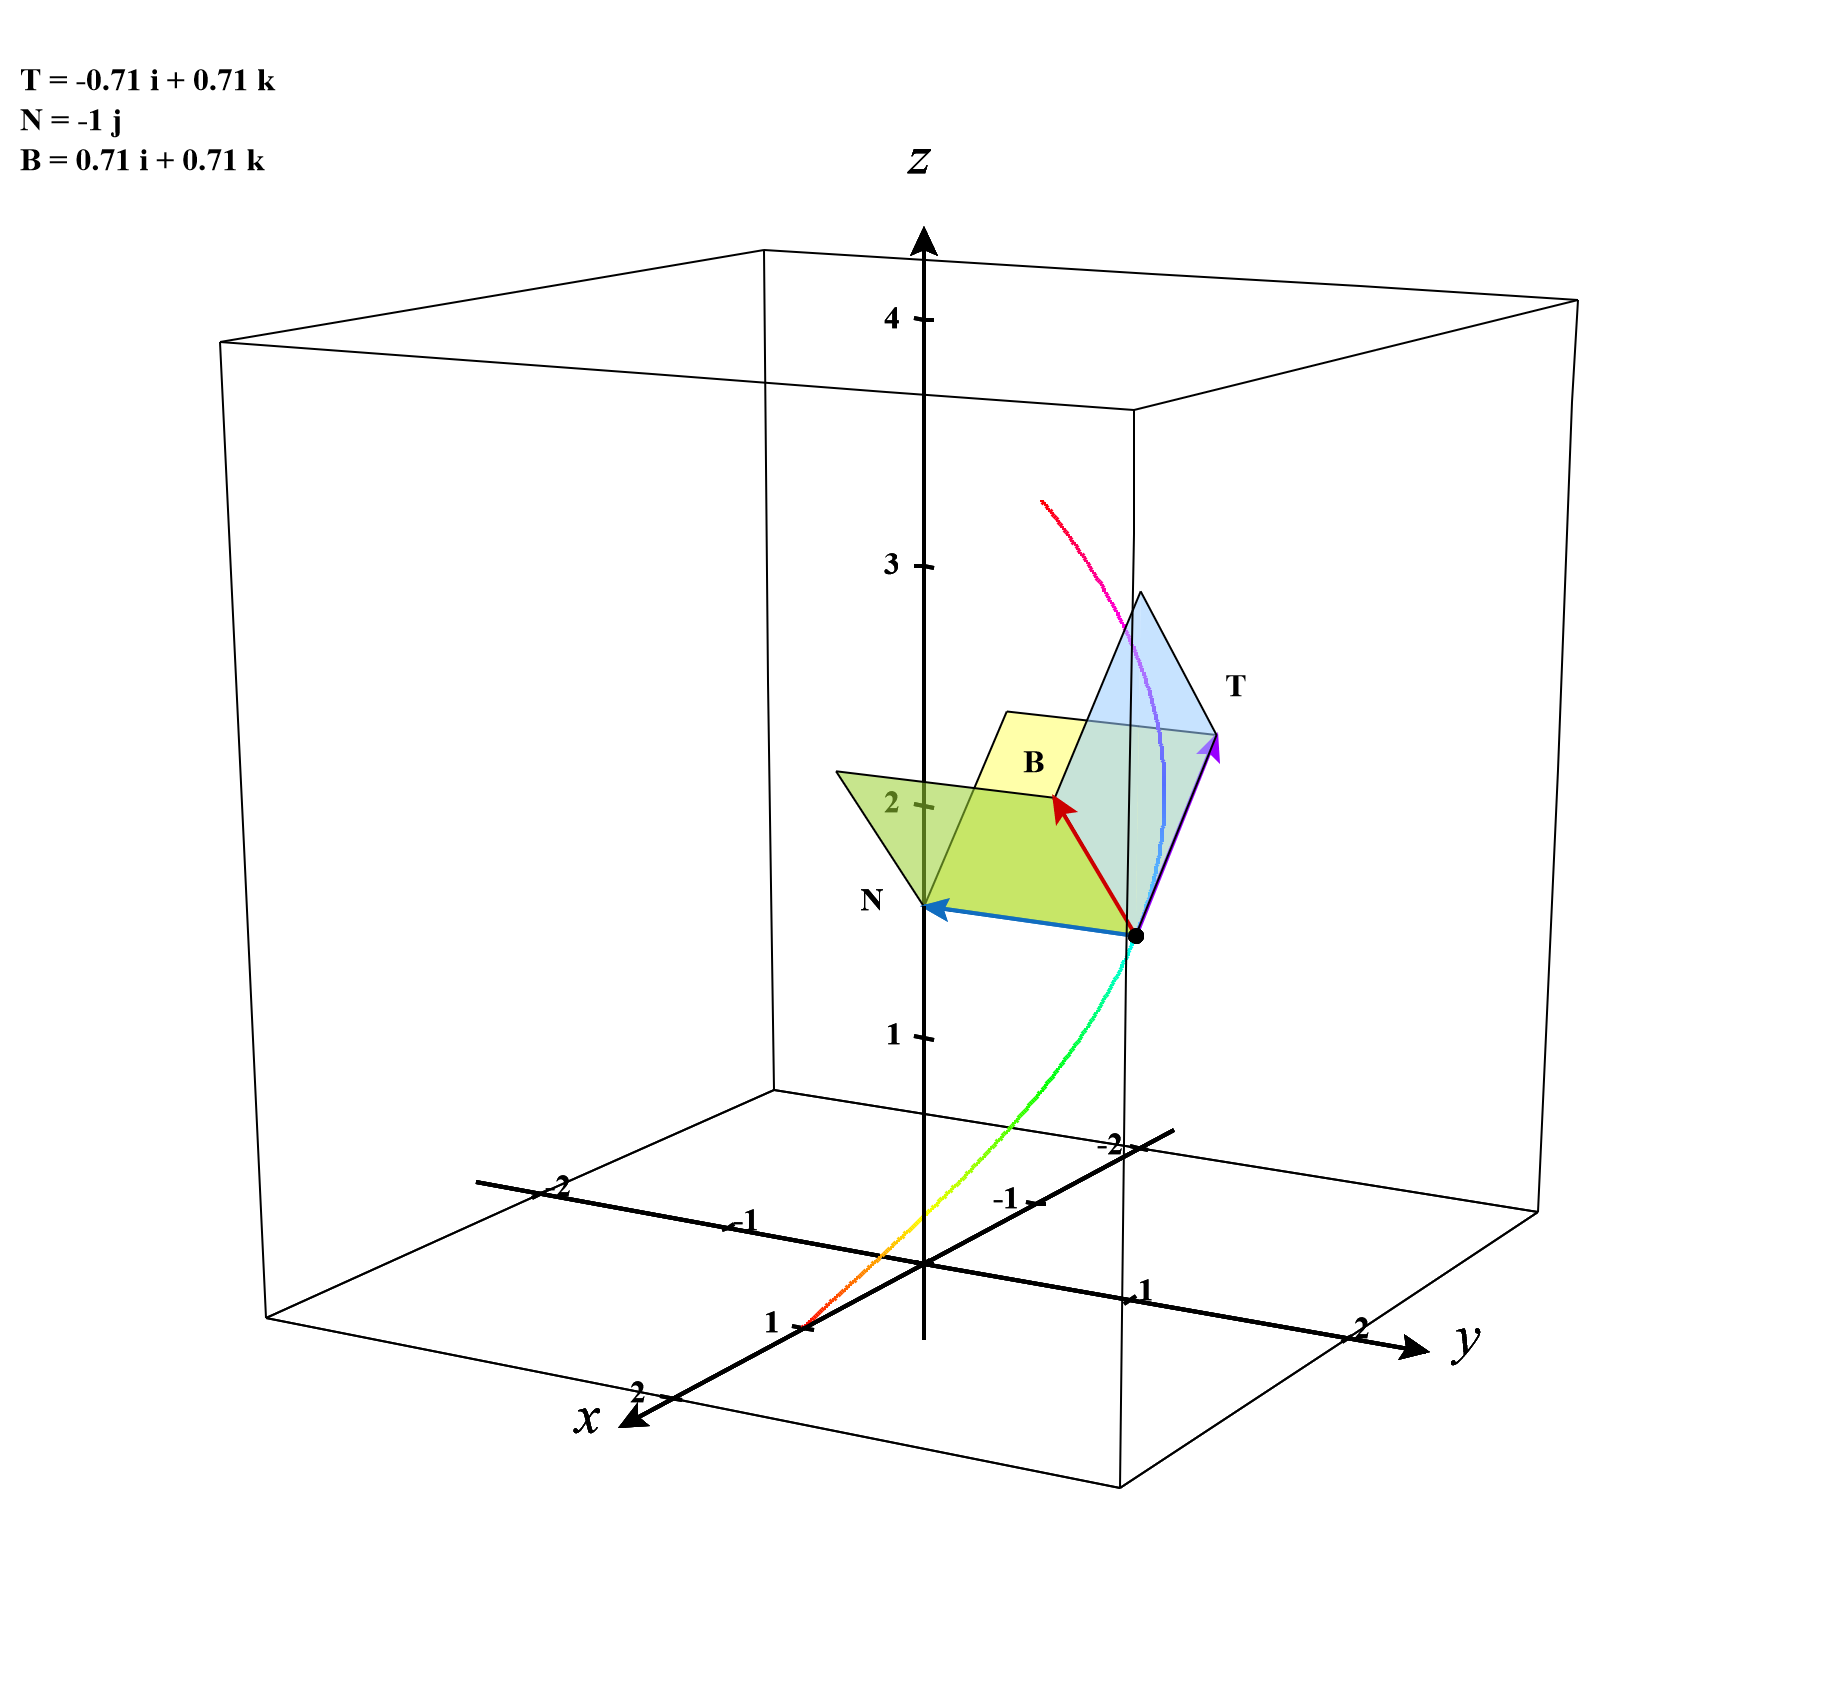
\includegraphics[width=0.85\textwidth]{../images/9-8-14.png}    
    \end{center}
    \end{red}
\end{enumerate}

\item (\href{https://activecalculus.org/multi/S-9-7-Vector-Valued-Functions-Derivatives.html#Ez_9_7_4}{AC Multi 9.7 Exercise 16})
For each given function $\vr$, determine $\int \vr(t)\, dt$. In addition, recalling the Fundamental Theorem of Calculus for functions of a single variable, also evaluate $\int_0^1 \vr(t)\, dt$ for each given function $r$. Is the resulting quantity a scalar or a vector? What does it measure?

\begin{red}
    If we label the antiderivative $\int\vr(t)\, dt$ as $\mathbf{R}(t)$, then $\int_0^1 \vr(t)\, dt$ will be a vector that points from $\mathbf{R}(0)$ to $\mathbf{R}(1)$. 
\end{red}

\begin{enumerate}
    \item $\displaystyle \vr(t) = \left\langle \cos(t), \frac{1}{t+1}, te^t \right\rangle$
    \begin{red}
        \begin{align*}
            \int\vr(t)\, dt &= \left\langle 
                \int\cos(t)\, dt, 
                \int\frac{1}{t+1}\, dt,
                \int te^t\, dt
            \right\rangle \\
            &= \left\langle
                \sin(t), 
                \ln|t+1|,
                t e^t - e^t
            \right\rangle + \vec{C} \\
            \int_0^1\vr(t)\, dt &= \left. \left\langle
                \sin(t), 
                \ln|t+1|,
                t e^t - e^t
            \right\rangle \right|_0^1 \\
            &= \left\langle
                \sin(1) - \sin(0),
                \ln(2) - \ln(1),
                (1e^1-e^1)-(0e^0 - e^0)
            \right\rangle
            = \left\langle
                \sin(1),
                \ln(2),
                1
            \right\rangle
        \end{align*}
    \end{red}
    \item $\displaystyle \vr(t) = \left\langle \cos(3t), \sin(2t), t \right\rangle$
    \begin{red}
        \begin{align*}
            \int\vr(t)\, dt &= \left\langle
                \frac13 \sin(3t),
                -\frac12 \cos(2t),
                \frac12 t^2
            \right\rangle +\vec{C} \\
            \int_0^1\vr(t)\, dt &= \left.\left\langle
                \frac13 \sin(3t),
                -\frac12 \cos(2t),
                \frac12 t^2
            \right\rangle \right|_0^1 \\
            &= \left\langle
                \frac13 \sin(3),
                -\frac12 (\cos(2) - 1),
                \frac12
            \right\rangle
        \end{align*}
    \end{red}
    \item $\displaystyle \vr(t) = \left\langle \frac{t}{1+t^2}, te^{t^2}, \frac{1}{1+t^2} \right\rangle$

    \begin{red}
        (The first two components require integration by substitution!)
        \begin{align*}
            \int\vr(t)\, dt &= \left\langle
                \frac12 \ln(1+t^2),
                \frac12 e^{t^2},
                \arctan(t)
            \right\rangle + \vec{C}\\
            \int\vr(t)\, dt &= \left.\left\langle
                \frac12 \ln(1+t^2),
                \frac12 e^{t^2},
                \arctan(t)
            \right\rangle \right|_0^1 \\
            &= \left\langle
                \frac12 \ln(2),
                \frac12 (e - 1),
                \frac{\pi}{4}
            \right\rangle
        \end{align*}
    \end{red}
\end{enumerate}

\item (\href{https://activecalculus.org/multi/S-9-7-Vector-Valued-Functions-Derivatives.html#Ez_9_7_5}{AC Multi 9.7 Exercise 17}) In this exercise, we develop the formula for the position function of a projectile that has been launched at an initial speed of $|\vv_0|$ and a launch angle of $\theta$. Recall that $\va(t) = \langle 0, -g\rangle$ is the constant acceleration of the projectile at any time $t$.
\begin{enumerate}
    \item Find all velocity vectors for the given acceleration vector $\va(t)$. When you anti-differentiate, remember that there is an arbitrary constant that arises in each component.
    \begin{red}
        \begin{equation*}
            \vv(t) = \int \va(t)\, dt = \left\langle
                \int 0\, dt,
                \int -g\, dt
            \right\rangle
            = \left\langle
                c_1, -gt + c_2
            \right\rangle
        \end{equation*}
    \end{red}
    \item Use the given information about initial speed and launch angle to find $\vv_0$, the initial velocity of the projectile. You will want to write the vector in terms of its components, which will involve $\sin\theta$ and $\cos\theta$.
    \begin{red}
        \begin{equation*}
            \vv_0 = 
            \left\langle |\vv_0|\cos\theta, |\vv_0|\sin\theta \right\rangle 
        \end{equation*}
    \end{red}
    \item Next, find the specific velocity vector function $\vv(t)$ for the projectile. That is, combine your work in (a) and (b) in order to determine expressions in terms of $|\vv_0|$ and $\theta$ for the constants that arose when integrating.

    \begin{red}
        On the one hand, $\vv_0 = \left\langle |\vv_0|\cos\theta, |\vv_0|\sin\theta \right\rangle$. But on the other hand, $\vv_0 = \vv(0) = \left\langle c_1, c2 \right\rangle$. 
        Therefore, $c_1 = |\vv_0|\cos\theta$ and $c_2 = |\vv_0|\sin\theta$. So,
        \[\vv(t) = \left\langle |\vv_0|\cos\theta, -gt + |\vv_0|\sin\theta \right\rangle.\]
    \end{red}
    \item Find all possible position vectors for the velocity vector $\vv(t)$ you determined in (c).
    \begin{red}
        \begin{align*}
            \vr(t) = \int \vv(t)\, dt &= \left\langle \int |\vv_0|\cos\theta\, dt, \int -gt + |\vv_0|\sin\theta\,dt \right\rangle \\
            &= \left\langle
                (|\vv_0|\cos\theta)t + c_3, 
                -\frac{g}{2} t^2 + (|\vv_0|\sin\theta )t + c_4
            \right\rangle
        \end{align*}
    \end{red}
    \item Let $\vr(t)$ denote the position vector function for the given projectile. Use the fact that the object is fired from the position $(x_0, y_0)$ to show it follows that
    \begin{equation*}
        \vr(t) = \left\langle |\vv_0| \cos(\theta)t + x_0, -\frac{g}{2}t^2 + |\vv_0| \sin(\theta)t + y_0 \right\rangle.
    \end{equation*}
    
    \begin{red}
        On the one hand, 
        \[\vr(0) = \left\langle
            (|\vv_0|\cos\theta)\cdot 0 + c_3, 
            -\frac{g}{2}\cdot  0^2 + (|\vv_0|\sin\theta )\cdot 0 + c_4
        \right\rangle = \left\langle c_3, c_4\right\rangle.\]
        On the other hand, $\vr(0) = \vr_0 = \left\langle x_0, y_0 \right\rangle$. 
        Therefore, $c_3 = x_0$ and $c_4 = y_0$; plugging those in gives us the requested thing, yay!
    \end{red}
\end{enumerate}

\item (\href{https://activecalculus.org/multi/S-9-8-Arc-Length-Curvature.html#Ez_9_8_1}{AC Multi 9.8 Exercise 11}) Consider the moving particle whose position at time $t$ in seconds is given by the vector-valued function $\vr$ defined by $\vr(t) = 5t \vi + 4\sin(3t) \vj + 4\cos(3t) \vk$.
\begin{enumerate}
    \item Find the unit tangent vector, $\vT(t)$, to the space curve traced by $\vr(t)$ at time $t$. Write one sentence that explains what $\vT(t)$ tells us about the particle's motion.
    \begin{red}
        \begin{align*}
            \vr'(t) &= \left\langle 5, 12 \cos(3t), -12\sin(3t) \right\rangle\\
            |\vr'(t)| &= \sqrt{
                5^2 + 144 \cos^2(3t) + 144 \sin^2(3t) 
            }
            = \sqrt{25 + 144} = \sqrt{169} = 13 \\
            \vT(t) = \dfrac{\vr'(t)}{|\vr'(t)|} &= \left\langle
                \frac{5}{13},
                \frac{12\cos(3t)}{13},
                -\frac{12 \sin(3t)}{13}
            \right\rangle
        \end{align*}
        $\vT(t)$ is a unit vector pointing in the direction the particle is moving at any particular time $t$.
    \end{red}
    \item Determine the speed of the particle moving along the space curve with the given parameterization.
    
    \begin{red}
        The speed of the particle is the magnitude of the velocity, which we've happily already computed:
        \[ |\vr'(t)| = \sqrt{
            5^2 + 144 \cos^2(3t) + 144 \sin^2(3t) 
        }
        = \sqrt{25 + 144} = \sqrt{169} = 13 \]
        (So in fact this particle is moving at constant speed.)
    \end{red}
    \item Find the exact distance traveled by the particle on the time interval $[0, \pi/3]$.

    \begin{red}
        Arc length = $\displaystyle \int_0^{\pi/3} |\vr'(t)| \, dt
        = \int_0^{\pi/3} 13\, dt = \dfrac{13\pi}{3}$
    \end{red}
    \item Find the average velocity of the particle on the time interval $[0, \pi/3]$.

    \begin{red}
        The average velocity is the total distance traveled divided by the total time elapsed, which you will certainly agree is $13$.
    \end{red}
    \item Determine the parameterization of the given curve with respect to arc length.

    \begin{red}
        Since the speed of the particle is constant, to achieve a parameterization that travels at unit speed, we need only divide by the constant speed:
        \[\vr(t) = \left\langle
            \frac{5t}{13}, \frac{4\sin(3t)}{13}, \frac{4\cos(3t)}{13}
        \right\rangle \]
    \end{red}
\end{enumerate}

\end{enumerate}
	
\end{document}